\chapter{EDA For Unstructured Data}


\section{Traffic Camera Image Analysis}
\begin{figure}[H]
  \centering
  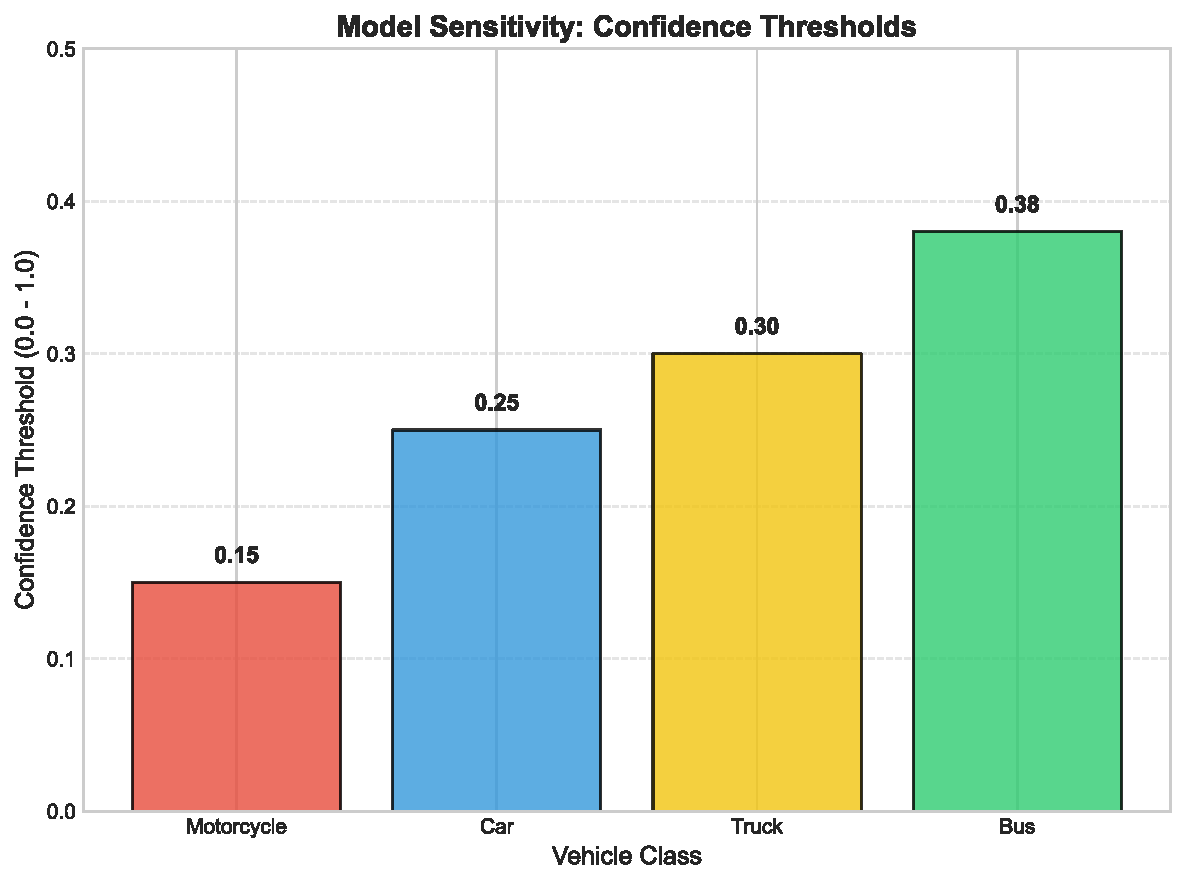
\includegraphics[width=0.8\textwidth]{figures/model_sensitivity.pdf} 
  \caption{Model Sensitivity Analysis}
\end{figure}
\begin{table}[h]
    \centering
    \caption{Optimized Detection Thresholds by Vehicle Class}
    \label{tab:thresholds}
    \begin{tabular}{|l|c|c|l|}
        \hline
        \textbf{Class} & \textbf{Threshold} & \textbf{Sensitivity} & \textbf{Objective} \\
        \hline
        Motorcycle & 0.15 & High & Maximize detection in dense/occluded traffic \\
        \hline
        Car & 0.25 & Medium & Standard detection baseline \\
        \hline
        Truck & 0.30 & Low & Reduce confusion with large passenger vehicles \\
        \hline
        Bus & 0.38 & Very Low & Ensure high precision for routing data integrity \\
        \hline
    \end{tabular}
\end{table}

\textbf{Analysis:} The motorcycle threshold is set aggressively low ($0.15$) to mitigate occlusion issues common in HCMC's mixed traffic flow. Conversely, the bus threshold is stringent ($0.38$) to prevent false positives from corrupting the public transport routing database.




\section{Traffic Congestion Data Pipeline}
\begin{figure}[H]
\centering
\begin{tikzpicture}[
    node distance=1.2cm and 1.5cm,
    % Define styles
    process/.style={
        rectangle, 
        minimum width=3.5cm, 
        minimum height=1cm, 
        text centered, 
        draw=black!70, 
        fill=blue!10, 
        rounded corners=3pt,
        drop shadow,
        font=\sffamily\footnotesize
    },
    data/.style={
        cylinder, 
        shape border rotate=90, 
        draw=black!70, 
        aspect=0.25, 
        fill=yellow!10, 
        minimum width=2cm, 
        minimum height=1.2cm, 
        align=center,
        drop shadow,
        font=\sffamily\scriptsize
    },
    file/.style={
        note, 
        draw=black!70, 
        fill=green!5, 
        align=center,
        drop shadow,
        font=\ttfamily\scriptsize,
        minimum width=2.5cm
    },
    % Define specific shapes for file icons if 'note' isn't available, using rectangle for simplicity
    file_rect/.style={
        rectangle,
        draw=black!60,
        fill=green!5,
        text width=4cm,
        align=center,
        minimum height=1cm,
        drop shadow,
        font=\ttfamily\scriptsize
    },
    arrow/.style={thick, -{Stealth[length=3mm]}, color=black!80},
    line/.style={thick, color=black!80}
]

% --- Nodes ---

% 1. Ingestion
\node (cameras) [process, fill=gray!20] {Camera Feeds / Images};
\node (detector) [process, below=of cameras, align=center] {\textbf{detector\_batch.py}\\(YOLOv11 Detection)};
\node (db) [data, below=of detector] {\textbf{detections.db}\\(Raw Detections)};

% 2. Mapping
\node (mapper) [process, below=of db, align=center] {\textbf{CameraToSegmentMapper}\\(Map GPS to Road)};
\node (segments) [file_rect, right=of mapper] {segments.csv};

% 3. Aggregation
\node (aggregator) [process, below=of mapper, align=center] {\textbf{SegmentAggregator}\\(Time Windowing)};
\node (agg_file) [file_rect, below=of aggregator] {segment\_aggregated.csv};

% 4. Thresholds (Branch)
\node (thresh_calc) [process, left=of agg_file, xshift=-0.5cm, align=center] {\textbf{ThresholdCalc}\\(Percentile Logic)};
\node (thresh_file) [file_rect, below=of thresh_calc] {segment\_thresholds.json};

% 5. Classification
\node (classifier) [process, below=of agg_file, yshift=-1.5cm, text width=3.5cm, align=center] {\textbf{CongestionClassifier}\\(Classify \& Update)};
\node (geo_in) [file_rect, right=of classifier] {segment\_geometries.geojson\\(Input Map)};
\node (geo_out) [file_rect, below=of classifier] {\textbf{final\_congestion.geojson}\\(Visualization Ready)};

% --- Edges ---

% Ingestion Flow
\draw [arrow] (cameras) -- (detector);
\draw [arrow] (detector) -- (db);

% Mapping Flow
\draw [arrow] (db) -- (mapper);
\draw [arrow] (mapper) -- (segments);

% Aggregation Flow
\draw [arrow] (db) to [bend right=45] (aggregator.north west);

\draw [arrow] (segments) -- (aggregator.east);
\draw [arrow] (aggregator) -- (agg_file);

% Threshold Branch
\draw [arrow] (agg_file) -- (thresh_calc.east);
\draw [arrow] (thresh_calc) -- (thresh_file);

% Classification Flow
\draw [arrow] (agg_file) -- (classifier);
\draw [arrow] (thresh_file) |- (classifier);
\draw [arrow] (geo_in) -- (classifier);
\draw [arrow] (classifier) -- (geo_out);

% Labels for steps
\node [right=0.2cm of detector, font=\scriptsize\itshape, text=gray] {Step 1: Detect};
\node [left=0.2cm of mapper, font=\scriptsize\itshape, text=gray] {Step 2: Map};
\node [left = 0.2cm of aggregator, font=\scriptsize\itshape, text=gray] {Step 3: Aggregate};
\node [right=0.25 of classifier, font=\scriptsize\itshape, text=gray, yshift=-1cm] {Step 4: Classify};
\end{tikzpicture}
\caption{Traffic Congestion Data Pipeline Architecture}
\end{figure}
